\documentclass[12pt, a4paper, oneside]{ctexart}
\usepackage{amsmath, amsthm, amssymb, bm, color, framed, graphicx, hyperref, mathrsfs,enumerate}

\title{\textbf{微分几何大作业}}
\author{2022数学萃英班\qquad 王一鑫}
\date{\today}
\linespread{1.5}
\definecolor{shadecolor}{RGB}{241, 241, 255}
\newcounter{problemname}
\newenvironment{problem}{\begin{shaded}\stepcounter{problemname}\par\noindent\textbf{题目\arabic{problemname}. }}{\end{shaded}\par}
\newenvironment{solution}{\par\noindent\textbf{解答. }}{\hfill$\qed$\par}
\newenvironment{note}{\par\noindent\textbf{题目\arabic{problemname}的注记. }}{\par}
\renewcommand{\parallel}{\mathrel{/\mskip-4mu/}}

\begin{document}
	
	\maketitle
	\begin{problem}
		向量积的概念可以推广到高维空间吗?
	\end{problem}
	
	\begin{solution}
		
		在Wikipedia中,我查询到了有关\textbf{七维向量积}的信息. 
		
		七维向量积是七维空间中向量的双线性算子,和三维向量积有着类似的性质:
		\begin{itemize}
			\item 满足反交换律.
			\item 对于$\mathbf{a}, \mathbf{b}\in \mathbb{R}^{7},\ \mathbf{a}\times\mathbf{b}$与$\mathbf{a}$和$\mathbf{b}$正交.
		\end{itemize}
		然而,也有不同的特性:
		\begin{itemize}
			\item 七维向量积不满足Jacobi恒等式.
			\item 每对三维向量只有一个向量积(不考虑正负),每对七维向量可以有很多向量积.
		\end{itemize}
		具体定义如下:在Euclidean空间 $V$ 上的向量积是一种双线性映射(bilinear map),将 $V$ 中的向量 $\bm{x}$ 和 $\bm{y}$ 映射到 $V$ 中的另一个向量 $\bm{x} \times \bm{y}$,并具有以下性质:
		
		\begin{itemize}
			\item \textbf{正交性:}
			\[
			\bm{x} \cdot (\bm{x} \times \bm{y}) = (\bm{x} \times \bm{y}) \cdot \bm{y} = 0,
			\]
			
			\item \textbf{模长:}
			\[
			|\bm{x} \times \bm{y}|^2 = |\bm{x}|^2 |\bm{y}|^2 - \langle\bm{x}, \bm{y}\rangle^2,
			\]
			可以等价表达式为:
			\[
			|\bm{x} \times \bm{y}| = |\bm{x}| |\bm{y}| \sin \theta,
			\]
			这是以 $\bm{x}$ 和 $\bm{y}$ 为边所围成的平行四边形的面积。
			
			\item 
			\[
			|\bm{x} \times \bm{y}| = |\bm{x}| |\bm{y}| \quad \text{当} \ \langle\bm{x},\bm{y}\rangle = 0,
			\]
		\end{itemize}
		具体运算可以由乘法表给出. Cayley给出了如下的乘法表:
		\[
		\begin{array}{|c|c|c|c|c|c|c|c|}
			\hline
			\times & e_1 & e_2 & e_3 & e_4 & e_5 & e_6 & e_7 \\ \hline
			e_1 & 0 & e_3 & -e_2 & e_5 & -e_4 & -e_7 & e_6 \\ \hline
			e_2 & -e_3 & 0 & e_1 & e_6 & e_7 & -e_4 & -e_5 \\ \hline
			e_3 & e_2 & -e_1 & 0 & e_7 & -e_6 & e_5 & -e_4 \\ \hline
			e_4 & -e_5 & -e_6 & -e_7 & 0 & e_1 & e_2 & e_3 \\ \hline
			e_5 & e_4 & -e_7 & e_6 & -e_1 & 0 & -e_3 & e_2 \\ \hline
			e_6 & e_7 & e_4 & -e_5 & -e_2 & e_3 & 0 & -e_1 \\ \hline
			e_7 & -e_6 & e_5 & e_4 & -e_3 & -e_2 & e_1 & 0 \\ \hline
		\end{array}
		\]
		该表格可以用于计算任意两个向量的向量积. 例如,要计算 $\bm{x} \times \bm{y}$ 的 $\bm{e}_1$ 分量,可以选择出所有与 $\bm{e}_1$ 相关的基向量相乘项,结果为:
		\[
		(\bm{x} \times \bm{y})_1 = x_2 y_3 - x_3 y_2 + x_4 y_5 - x_5 y_4 + x_7 y_6 - x_6 y_7.
		\]这样的乘法表并不唯一.
		
		对于更一般的向量积推广,有如下结果:在任意维度内的 $r$ 元运算,可以通过某些公理实现。假设在一个 $d$ 维空间 $V$ 上存在一个 $r$ 元运算。于是,一个 $r$-重 $d$-维“向量积”多线性运算可以表示为:
		\[
		(C_1 \times C_2 \times \cdots \times C_r): V^{dr} = \underbrace{V^d \times \cdots \times V^d}_{r} \to V^d
		\]
		
		满足以下性质:
		\[
		\forall i = 1, 2, \ldots, r
		\]
		\[
		(C_1 \times C_2 \times \cdots \times C_r) \cdot C_i = 0
		\]
		
		并且:
		\[
		(C_1 \times C_2 \times \cdots \times C_r) \cdot (C_1 \times C_2 \times \cdots \times C_r) = \det(C_i \cdot C_j)
		\]
		
		Eckmann(1943)和 Whitehead(1963)解决了实欧几里得空间中连续情况的问题,而 Brown 和 Gray(1967)解决了多线性情况。此外,该解法对任意特征不为 $2$ 的域都适用,并且适用于 $1 \leq r \leq d$ 的情况。定理(Eckmann、Whitehead 和 Brown-Gray 的结果)表明,只有在以下条件下,“广义向量积”才存在:
		\begin{enumerate}[(1)]
			\item $d$ 为偶数,$r = 1$
			
			在每一个偶数维度中,单一因子的向量积存在. 这可以被视为某种“Wick 旋转”.
			\item $d$ 是任意值,$r = d - 1$
			
			在任意维度 $d$ 中,$(d-1)$-重向量积是存在的. 只需取这些 $(d-1)$ 个向量与标准正交基向量 $(e_1, \ldots, e_r)$ 的行列式即可.
			
			\item $d = 3, 7$,$r = 2$
			在$3$维和$7$维空间中存在$2$重向量积.正是我们熟知的向量积与刚才所提到的七维向量积.
	
			\item $d = 8$,$r = 3$
			在$8$维空间中存在$3$重向量积.
		\end{enumerate}
		。
	\end{solution}
	\begin{problem}
		将Gauss映射推广到$3$维和$4$维空间的曲线上.
	\end{problem}
	
	\begin{solution}
		回顾$2$维空间曲线$\mathbf{r}$的Gauss映射. 在曲线$\mathbf{r}$的任一点$\mathbf{r}(s)$,有一个单位法向量$\mathbf{n}(s)$,将$\mathbf{n}(s)$的起点平移到平面的原点,$\mathbf{n}(s)$的终点就落到单位圆周$S^{1}$上,这样就定义了一个映射\[ \begin{aligned}
			g: \mathbf{r}&\rightarrow S^{1}\\ s&\mapsto\mathbf{n}(s)
		\end{aligned} \]
		\begin{center}
			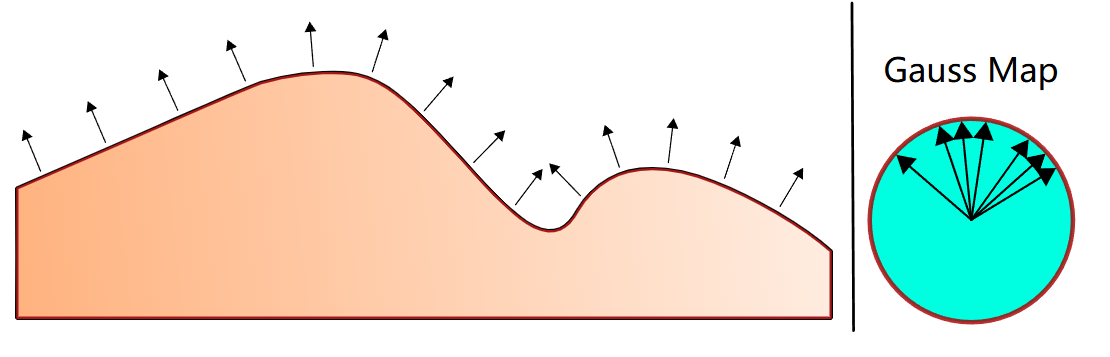
\includegraphics[width=0.75\textwidth]{pics/figure2.png} 
		\end{center}
		在$3$维空间中,对于曲面$S$上的一条正则曲线,每一点都有确定的法向量. 类似地,将法向量的起点平移到原点,法向量就落到单位球面$S^{2}$上.
		
		在$4$维甚至更高维的$R^{n}$中的超曲面中,给出$R^{n}$中的曲面$S$,高斯映射是一个连续映射\[ g: S\rightarrow S^{n-1} \]使得$g(p)$是在点$p$上正交于$S$的单位向量,即曲面$S$在点$p$处的法向量.从超曲面映射到$R^{n}$中的单位球面$S^{n-1}$.
	\end{solution}
	
	\begin{problem}
		证明:正螺旋面$\mathbf{r}(u,v) = (u\cos v, u\sin v, bv)$是极小曲面;并证明:直纹极小曲面是平面或者正螺旋面. 
	\end{problem}
	\begin{center}
		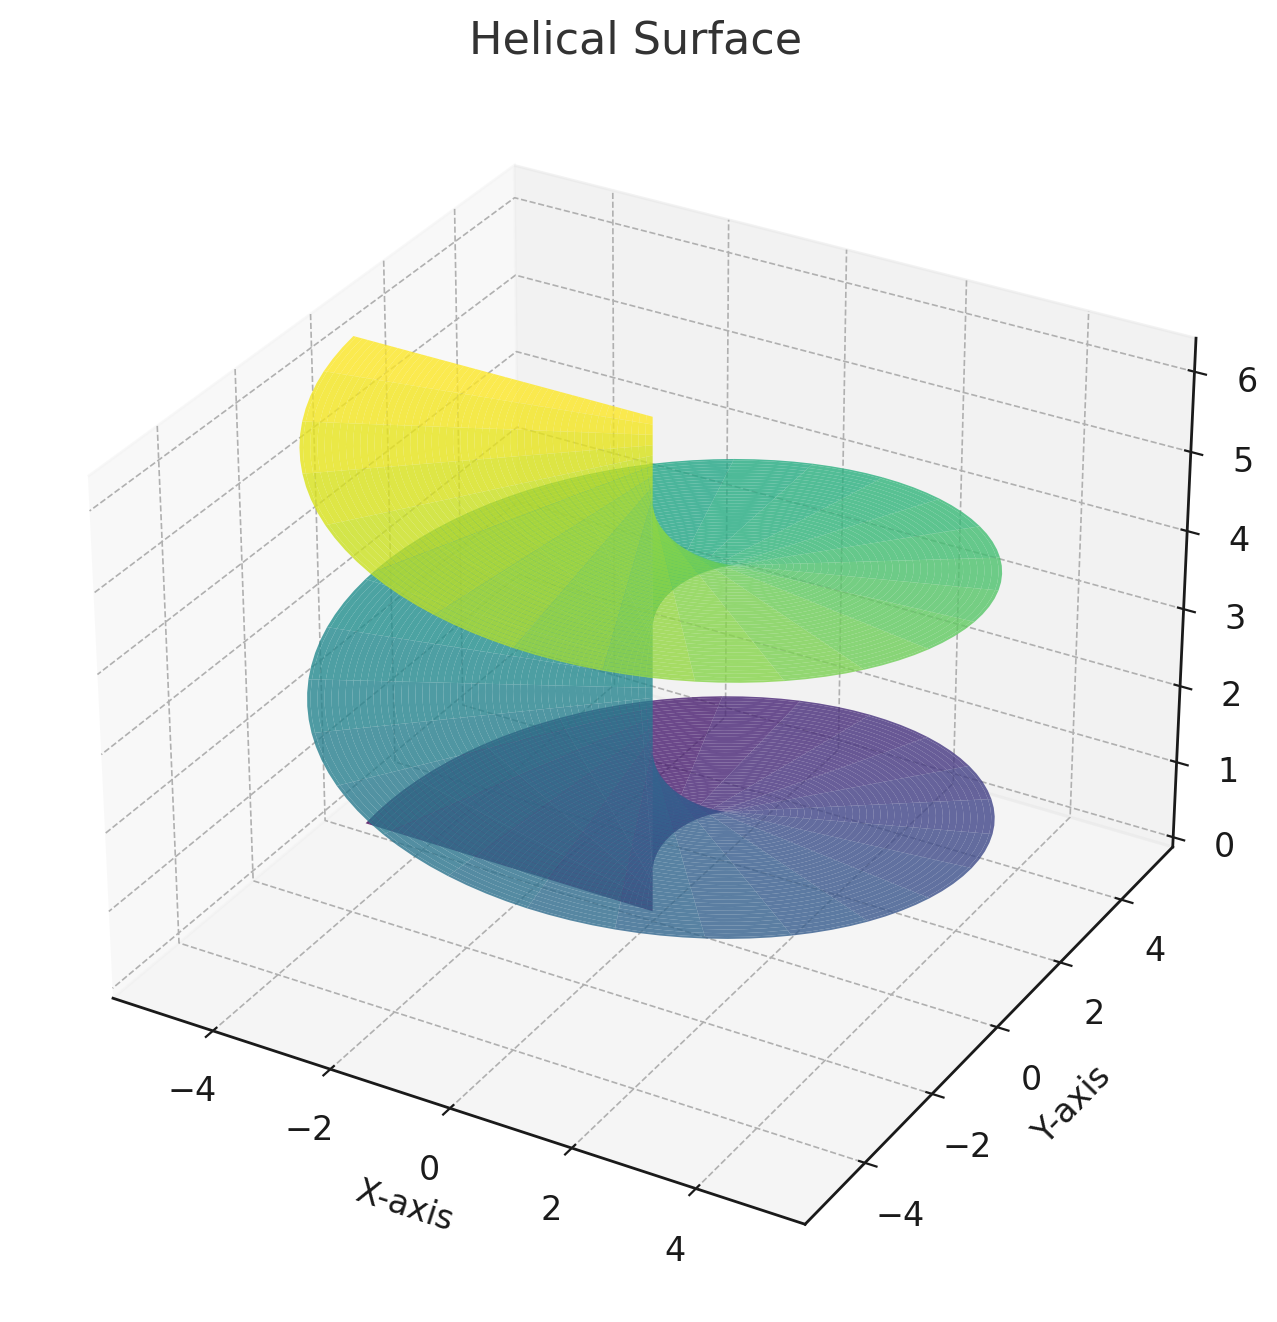
\includegraphics[width=0.5\textwidth]{pics/figure1.png} 
	\end{center}
	
	\begin{solution}
		直接计算,有
		\[
		\mathbf{r}_{u} = (\cos v, \sin v, 0), \quad \mathbf{r}_{v} = (-u \sin v, u \cos v, b),
		\]
		\[
		\mathbf{n} = \frac{1}{\sqrt{u^2 + b^2}}(b \sin v, -b \cos v, u).
		\]
		
		故
		\[
		E = 1, \quad F = 0, \quad G = u^2 + b^2.
		\]
		
		又
		\[
		\mathbf{r}_{uu} = 0, \quad \mathbf{r}_{uv} = (-\sin v, \cos v, 0), \quad \mathbf{r}_{vv} = (-u \cos v, -u \sin v, 0),
		\]
		
		故
		\[
		L = 0, \quad M = -\frac{b}{\sqrt{u^2 + b^2}}, \quad N = 0.
		\]
		
		从而,平均曲率
		\[
		H = \frac{LG - 2MF + NE}{2(EG - F^2)} = 0.
		\]
		
		由极小曲面定义,知正螺旋面是极小曲面.
		
		下证直纹极小曲面是平面或者正螺旋面. 设极小直纹面 $S$ 的参数表示为 $\mathbf{r}(u, v) = \mathbf{a}(u) + v\mathbf{b}(u)$,则
		\[
		\mathbf{r}_u = \mathbf{a}'(u) + v\mathbf{b}'(u), \quad \mathbf{r}_v = \mathbf{b}(u), \quad \mathbf{r}_u \wedge \mathbf{r}_v = \mathbf{a}'(u) \wedge \mathbf{b}(u) + v\mathbf{b}'(u) \wedge \mathbf{b}(u).
		\]
		
		故
		\[
		E = \langle \mathbf{a}', \mathbf{a}' \rangle + 2v \langle \mathbf{a}', \mathbf{b}' \rangle + v^{2}\langle \mathbf{b}', \mathbf{b}'\rangle, \quad F = \langle\mathbf{a}', \mathbf{b}\rangle + v \langle \mathbf{b}', \mathbf{b} \rangle, \quad G = \langle \mathbf{b}, \mathbf{b} \rangle.
		\]
		
		作参数变换使得$(u,v)$是正交参数,从而$|\mathbf{b}(u)| = 1$,以及$\langle \mathbf{a}'(u), \mathbf{b}(u) \rangle = 0$.此时$F = 0,\, G = 1$.
		
		由
		\[
		\mathbf{r}_{uu} = \mathbf{a}'' + v \mathbf{b}''(u), \quad \mathbf{r}_{uv} = \mathbf{b}'(u), \quad \mathbf{r}_{vv} = 0,
		\]
		
		记$\Delta:=|\mathbf{r}_{u}\wedge\mathbf{r}_{v}|$. 计算得
		\[\begin{aligned}
			L = \frac{1}{\Delta} \Big[( \mathbf{a}'', \mathbf{a}', \mathbf{b})  &+ v \big(( \mathbf{a}', \mathbf{b}, \mathbf{b}'' ) +  (\mathbf{a}'', \mathbf{b}', \mathbf{b})\big) + v^2 (\mathbf{b}'', \mathbf{b}', \mathbf{b})\Big]\\ M &= \frac{1}{\Delta}(\mathbf{a}', \mathbf{b}, \mathbf{b}')\quad  N = 0
		\end{aligned}
		\]
		曲面 $S$ 是极小的 $\Leftrightarrow H = 0$,即
		\[
		0 = \Delta (L G - 2 M F + N E) = ( \mathbf{a}'', \mathbf{a}', \mathbf{b})  + v \big(( \mathbf{a}', \mathbf{b}, \mathbf{b}'' ) +  (\mathbf{a}'', \mathbf{b}', \mathbf{b})\big) + v^2 (\mathbf{b}'', \mathbf{b}', \mathbf{b}).
		\]
		
		等式成立当且仅当
		\[
		\begin{cases}
			( \mathbf{a}'', \mathbf{a}', \mathbf{b}) = 0 \\
			( \mathbf{a}', \mathbf{b}, \mathbf{b}'' ) +  (\mathbf{a}'', \mathbf{b}', \mathbf{b}) = 0 \\
			(\mathbf{b}'', \mathbf{b}', \mathbf{b}) = 0.\tag{*}
		\end{cases}
		\]
		
		由式(*)中第三式,知$\mathbf{b}(u)$ 在某个平面上,由假设 $|\mathbf{b}(u)| = 1$是一条单位球面曲线. 从而 $\mathbf{b}(u)$ 是一个单位圆.
		
		若 $\mathbf{a}(u)$ 为常向量,则 $S$ 是平面. 现在假设 $\mathbf{a}(u)$ 不为常向量. 可以设$u$是曲线$\mathbf{a}(u)$的弧长参数,它的Frenet标架为$\{\mathbf{a}(u), \mathbf{t}(u), \mathbf{n}(u), \mathbf{B}(u)\}$. 由(*)中第一式知\[ 0 = ( \mathbf{a}'', \mathbf{a}', \mathbf{b}) = (k\mathbf{n}, \mathbf{t}, \mathbf{b}) = -k\langle\mathbf{B},\mathbf{b}\rangle\]若$k=0$,则$\mathbf{a}(u)$是直线. 可以设
		\[
		\mathbf{a}(u) = (0, 0, bu).
		\]
		由假设及$\langle \mathbf{a}', \mathbf{b} \rangle = \langle \mathbf{t}, \mathbf{b} \rangle =0$,即$\mathbf{t}\perp \mathbf{b}$,故
		\[
		\mathbf{b}(u) = (\cos u, \sin u, 0).
		\]
		从而,曲面 $S$ 的参数表达式为
		\[
		\mathbf{r}(u, v) = \mathbf{a}(u) + v \mathbf{b}(u) = (v \cos u, v \sin u, bu).
		\]
		即,曲面 $S$ 为正螺旋面.
		
		若 $k$ 不恒等于$0$则$\langle\mathbf{B},\mathbf{b}\rangle=0$. 由假设 $\langle \mathbf{t}, \mathbf{b} \rangle =0$,于是$\mathbf{b}\parallel\mathbf{n}$. 不妨设$\mathbf{b} = \mathbf{n}$,由(*)中的第二式,有\begin{align*}
			0 &=  ( \mathbf{a}', \mathbf{b}, \mathbf{b}'' ) +  (\mathbf{a}'', \mathbf{b}', \mathbf{b})\\ &= (\mathbf{t}, \mathbf{n}, \ddot{\mathbf{n}}) + (\dot{\mathbf{t}}, \dot{\mathbf{n}}, \mathbf{n})\\ &=\langle \mathbf{B}, -\dot{k}\mathbf{t} - k^{2}\mathbf{n} + \dot{\tau}\mathbf{B} - \tau^{2}\mathbf{n}\rangle \\ &=\dot{\tau}
		\end{align*} 
		这表示$\tau$是常数.
		
		若$\tau\equiv0$,则$\mathbf{a}(u)$是平面曲线,$\mathbf{b}(u)$是其主法向量,从而$S$是平面.
		
		若$\tau\neq0$,则由(*)第三式知\[ 0 = (\mathbf{b}'', \mathbf{b}', \mathbf{b}) = (\ddot{\mathbf{n}}, \dot{\mathbf{n}}, \mathbf{n}) =  \dot{k}\tau\]因此$\dot{k} = 0$,即$k$为常数. 于是$\mathbf{a}(u)$是圆柱螺旋线,可设\[
		\mathbf{a}(u) = 
		\left(
		\frac{k}{k^2 + \tau^2} \cos\left(\sqrt{k^2 + \tau^2} u\right),
		\frac{k}{k^2 + \tau^2} \sin\left(\sqrt{k^2 + \tau^2} u\right),
		\frac{\tau}{\sqrt{k^2 + \tau^2}} u
		\right),
		\]
		
		则
		\[
		\mathbf{b}(u) = \mathbf{n}(u) = 
		\left(
		-\cos\left(\sqrt{k^2 + \tau^2} u\right),
		-\sin\left(\sqrt{k^2 + \tau^2} u\right),
		0
		\right).
		\]
		
		故
		\begin{align*}
			\mathbf{r}(u, v) &= \mathbf{a}(u) + v \mathbf{b}(u) \\&= 
			\left(
			\left(\frac{k}{k^2 + \tau^2} - v\right) \cos\left(\sqrt{k^2 + \tau^2} u\right),
			\left(\frac{k}{k^2 + \tau^2} - v\right) \sin\left(\sqrt{k^2 + \tau^2} u\right),
			\frac{\tau}{k^2 + \tau^2} u
			\right).
		\end{align*}
		
		作参数变换
		\[
		\tilde{v} = \sqrt{k^2 + \tau^2} u, \quad \tilde{u} = \frac{k}{k^2 + \tau^2} - v,
		\]
		
		则曲面 $S$ 的参数表达式变为
		\[
		\mathbf{r}(\tilde{u}, \tilde{v}) = 
		\left(
		\tilde{u} \cos \tilde{v},
		\tilde{u} \sin \tilde{v},
		\frac{\tau}{k^2 + \tau^2} \tilde{v}
		\right).
		\]
		
		故曲面 $S$ 是正螺旋面。
	\end{solution}
	
	
	\begin{problem}
		求$k_{n} = Lx^{2}+2Mxy + Ny^{2}$在约束\[ (x,y)\in\{(x,y)|Ex^{2}+2Fxy+Gy^{2}=1\} \]下的最大、最小值.
	\end{problem}
	
	\begin{solution}
		利用拉格朗日乘数法,构造拉格朗日函数:
		\[
		\mathcal{L}(x, y, \lambda) = Lx^2 + 2Mxy + Ny^2 - \lambda (Ex^2 + 2Fxy + Gy^2 - 1).
		\]
		
		$\mathcal{L}$ 分别对 $x$, $y$和 $\lambda$ 求偏导,并令偏导数等于$0$,得到以下方程:
		\begin{enumerate}[(i)]
			\item 对 $x$ 求偏导:
			\[
			\frac{\partial \mathcal{L}}{\partial x} = 2Lx + 2My - \lambda (2Ex + 2Fy) = 0,
			\]
			即:
			\[
			Lx + My = \lambda (Ex + Fy).
			\]
			
			\item  对 $y$ 求偏导:
			\[
			\frac{\partial \mathcal{L}}{\partial y} = 2Mx + 2Ny - \lambda (2Fx + 2Gy) = 0,
			\]
			即:
			\[
			Mx + Ny = \lambda (Fx + Gy).
			\]
			
			\item  对 $\lambda$ 求偏导:
			\[
			\frac{\partial \mathcal{L}}{\partial \lambda} = -(Ex^2 + 2Fxy + Gy^2 - 1) = 0,
			\]
			即:
			\[
			Ex^2 + 2Fxy + Gy^2 = 1.
			\]
		\end{enumerate}
		

		改写为矩阵形式:
		\[
		\begin{bmatrix}
			L - \lambda E & M - \lambda F \\
			M - \lambda F & N - \lambda G
		\end{bmatrix}
		\begin{bmatrix}
			x \\
			y
		\end{bmatrix}
		= \begin{bmatrix}
			0 \\
			0
		\end{bmatrix}.
		\]
		
		非零解 $(x, y)$ 存在的条件是系数矩阵的行列式为$0$:
		\[
		\det\begin{bmatrix}
			L - \lambda E & M - \lambda F \\
			M - \lambda F & N - \lambda G
		\end{bmatrix} = 0.
		\]
		展开得
		\[
		(L - \lambda E)(N - \lambda G) - (M - \lambda F)^2 = 0.
		\]
		
		展开后整理:
		\[
		\lambda^2 (EG - F^2) - \lambda (LG + NE - 2MF) + (LN - M^2) = 0. \tag{4}
		\]
		
		观察得与书中主曲率$k$满足的方程一致,记两个主曲率分别为$k_{1},k_{2}$且$k_{1}\geq k_{2}$.
		
		求得\[ \begin{aligned}
			(k_{n})_{\mathrm{max}} &= Lx^{2}+2Mxy + Ny^{2}\\ &= (Lx + My)x + (Mx + Ny)y\\ &= k_{1}(Ex+Fy)x + k_{1}(Fx+Gy)y \\&= k_{1}(Ex^{2}+2Fxy+Gy^{2}) = k_{1}
		\end{aligned} \]
		以及\[ \begin{aligned}
			(k_{n})_{\mathrm{min}} &= Lx^{2}+2Mxy + Ny^{2}\\ &= (Lx + My)x + (Mx + Ny)y\\ &= k_{2}(Ex+Fy)x + k_{2}(Fx+Gy)y \\&= k_{2}(Ex^{2}+2Fxy+Gy^{2}) = k_{2}
		\end{aligned} \]
	\end{solution}
	
	
	\begin{problem}
		验证\[ \frac{\partial b_{\alpha \beta}}{\partial u^{\gamma}} - \frac{\partial b_{\alpha \gamma}}{\partial u^{\beta}} + \Gamma^\xi_{\alpha \beta} b_{\xi \gamma} - \Gamma^\xi_{\alpha \gamma} b_{\xi \beta} = 0
		 \]和\[ \frac{\partial b^\xi_\beta}{\partial u^\gamma} - \frac{\partial b^\xi_\gamma}{\partial u^\beta} = - b^\eta_\beta \Gamma^\xi_{\eta \gamma} + b^\eta_\gamma \Gamma^\xi_{\eta \beta}
		  \]是等价的
	\end{problem}
	\begin{solution}
		回顾张量运算的性质,有\[ \Gamma_{\xi\alpha\beta} = g_{\gamma\xi}\Gamma_{\alpha\beta}^{\gamma}\quad b_{\alpha}^{\beta}  = b_{\alpha\gamma}g^{\gamma\beta} \]
		计算$g_{\alpha\xi}(\frac{\partial b^\xi_\beta}{\partial u^\gamma}+b^\eta_\beta \Gamma^\xi_{\eta \gamma})$会发现
		\[ \begin{aligned}
			g_{\alpha\xi}\Big(\frac{\partial b^\xi_\beta}{\partial u^\gamma}+b^\eta_\beta \Gamma^\xi_{\eta \gamma}\Big) &= \frac{\partial (b_{\beta\alpha}g^{\alpha\xi})}{\partial u^\gamma}g_{\alpha\xi} + b^\eta_\beta \Gamma{\alpha\eta \gamma}\\ &= \frac{\partial b_{\alpha\beta}}{\partial u^\gamma}g^{\alpha\xi}g_{\alpha\xi} + \frac{\partial g^{\alpha\xi}}{\partial u^\gamma}b_{\beta\alpha}g_{\alpha\xi} + b^\eta_\beta \Gamma{\alpha\eta \gamma}\\ &= \frac{\partial b_{\alpha\beta}}{\partial u^\gamma} - \frac{\partial g_{\alpha\xi}}{\partial u^\gamma}b_{\beta\alpha}g^{\alpha\xi} + b^\eta_\beta \Gamma{\alpha\eta \gamma}\\ &= \frac{\partial b_{\alpha\beta}}{\partial u^\gamma} + b_{\beta}^{\xi}\Big(\Gamma_{\alpha\xi\gamma} - \frac{\partial g_{\alpha\xi}}{\partial u^\gamma}\Big)\\ &= \frac{\partial b_{\alpha\beta}}{\partial u^\gamma} + b_{\beta}^{\xi}\Big[\dfrac{1}{2}\Big(\dfrac{\partial g_{\alpha\gamma}}{\partial u^{\xi}} + \dfrac{\partial g_{\alpha\beta}}{\partial u^{\gamma}} - \dfrac{\partial g_{\xi\gamma}}{\partial u^{\alpha}}\Big) - \dfrac{\partial g_{\alpha\beta}}{\partial u^{\gamma}}\Big]\\ &= \frac{\partial b_{\alpha\beta}}{\partial u^\gamma} - b_{\beta}^{\xi}\Gamma_{\xi\alpha\gamma}\\ &= \frac{\partial b_{\alpha\beta}}{\partial u^\gamma} - b_{\beta\eta}g^{\eta\xi}g_{\eta\xi}\Gamma_{\alpha\gamma}^{\eta}\\ &= \frac{\partial b_{\alpha\beta}}{\partial u^\gamma} - \Gamma_{\alpha\gamma}^{\xi}b_{\xi\beta}
		\end{aligned} \]
		同理,计算得\[ g_{\alpha\xi}\Big(\frac{\partial b^\xi_\gamma}{\partial u^\beta} + b^\eta_\gamma \Gamma^\xi_{\eta \beta}\Big) = \frac{\partial b_{\alpha \gamma}}{\partial u^{\beta}} - \Gamma^\xi_{\alpha \beta} b_{\xi \gamma}\]于是两式是等价的.
	\end{solution}
	
	\begin{problem}
		写出$F\neq0$时,Gauss曲率的内蕴(只由第一基本形式决定)计算公式.
	\end{problem}
	
	\begin{solution}
		当 $F \neq 0$ 时,
		
		假定曲面 $S$ 的第一基本形式为
		\[
		I = E \, du^2 + 2F \, du \, dv + G \, dv^2,
		\]
		即
		\[
		I = \left( \sqrt{E} \, du + \frac{F}{\sqrt{E}} \, dv \right)^2 + \left( \sqrt{\frac{EG - F^2}{E}} \, dv \right)^2.
		\]
		
		设 $g = EG - F^2$, 则
		\[
		\omega_1 = \sqrt{E} \, du + \frac{F}{\sqrt{E}} \, dv, \quad \omega_2 = \sqrt{\frac{g}{E}} \, dv.
		\]
		
		由 Gauss 的绝妙定理得
		\[
		K = -\frac{d\omega_{12}}{\omega_1 \wedge \omega_2}.
		\]
		
		计算得
		\[
		\omega_1 \wedge \omega_2 = \sqrt{g} \, du \wedge dv.
		\]
		
		设
		\[
		\omega_{12} = a \, \omega_1 \wedge \omega_1 + b \, \omega_1 \wedge \omega_2.
		\]
		
		由曲面的结构方程
		\[
		\begin{cases}
			d\omega_1 = \omega_{12} \wedge \omega_2, \\
			d\omega_2 = \omega_{21} \wedge \omega_1.
		\end{cases}
		\]
		
		由于
		\[
		d\omega_1 = d \left( \sqrt{E} \, du + \frac{F}{\sqrt{E}} \, dv \right) = \left[ -\frac{\partial \sqrt{E}}{\partial v} + \frac{\partial}{\partial u} \left( \frac{F}{\sqrt{E}} \right) \right] du \wedge dv,
		\]
		\[
		d\omega_2 = d \left( \sqrt{\frac{g}{E}} \, dv \right) = \frac{\partial}{\partial u} \left( \sqrt{\frac{g}{E}} \right) du \wedge dv.
		\]
		
		得
		\[
		a = \frac{1}{\sqrt{g}} \left[ -\frac{\partial \sqrt{E}}{\partial v} + \frac{\partial}{\partial u} \left( \frac{F}{\sqrt{E}} \right) \right],
		\]
		\[
		b = \frac{1}{\sqrt{g}} \frac{\partial}{\partial u} \left( \sqrt{\frac{g}{E}} \right).
		\]
		
		进而
		\[
		d\omega_{12} = d(a \, \omega_1 + b \, \omega_2) = d \left[ a \sqrt{E} \, du + a \frac{F}{\sqrt{E}} \, dv + b \sqrt{\frac{g}{E}} \, dv \right],
		\]
		\[
		= \left[ -\frac{\partial (a \sqrt{E})}{\partial v} + \frac{\partial}{\partial u} \left( a \frac{F}{\sqrt{E}} +b\sqrt{\dfrac{g}{E}}\right) \right] du \wedge dv.
		\]
		
		最后根据Gauss的绝妙定理
		\[
		K = -\frac{d\omega_{12}}{\omega_1 \wedge \omega_2},
		\]
		\begin{align*}
			K = &-\frac{1}{\sqrt{g}} \Bigg\{ 
			-\frac{\partial}{\partial v} \bigg[ \sqrt{\frac{E}{g}} \bigg( 
			-\frac{\partial \sqrt{E}}{\partial v} + \frac{\partial}{\partial u} 
			\Big( \frac{F}{\sqrt{E}} \Big) \bigg) \bigg] \\
			&\quad + \frac{\partial}{\partial u} \bigg[ \frac{F}{\sqrt{Eg}} \bigg( 
			-\frac{\partial \sqrt{E}}{\partial v} + \frac{\partial}{\partial u} 
			\Big( \frac{F}{\sqrt{E}} \Big) \bigg) \bigg] \\
			&\quad + \frac{\partial}{\partial u} 
			\bigg[ \frac{1}{\sqrt{E}} \cdot \frac{\partial}{\partial u} \Big( \sqrt{\frac{g}{E}} \Big) \bigg] 
			\Bigg\}.
		\end{align*}
		
	\end{solution}
	
	\begin{problem}
		求解二维非线性方程\[ -\Delta u = e^{2u} \]
	\end{problem}
	
	\begin{solution}
		曲面等温参数$(u,v)$下,曲面的第一基本形式为
		\[
		I = \lambda^2(u, v)(du \, du + dv \, dv), \quad \lambda \neq 0.
		\]
		根据Gauss的绝妙定理可以求得
		\[ 
		K = -\frac{1}{\lambda^2} \left( \frac{\partial^2}{\partial u^2} + \frac{\partial^2}{\partial v^2} \right) \ln \lambda.
		\] 
		令$u = \ln\lambda$,上式等价于
		\[ -\Delta u = Ke^{2u}  \]
		取$K = 1$. 考虑球极投影参数表示
		\[ \bm{r}(u,v) = \Big(2\dfrac{a^{2}u}{a^{2}+u^{2}+v^{2}}, 2\dfrac{a^{2}v}{a^{2}+u^{2}+v^{2}}, a\dfrac{u^{2}+v^{2}-a^{2}}{a^{2}+u^{2}+v^{2}}\Big) \]
		特别地,$a = 1$时,$K = 1$. 又
		\[ I(u,v) = \dfrac{4a^{4}}{(a^{2} + u^{2} + v^{2})^{2}}(\mathrm{d}u^{2} + \mathrm{d}v^{2}) \]
		可以求得\[ \lambda = \dfrac{2}{1 + u^{2} + v^{2}}\quad u = \ln\lambda = \ln\dfrac{2}{1 + u^{2} + v^{2}} \]
		
	\end{solution}
	
	\begin{problem}
		给出曲面$S$上的任意一条曲线$C$的测地曲率$k_{g}$一般的计算公式.
	\end{problem}
	\begin{solution}
		曲面 $S: \mathbf{r} = \mathbf{r}(u^1, u^2)$ 上任意一条曲线 $C: u^1 = u^1(s), u^2 = u^2(s)$ 作为空间 $E^3$ 中的曲线的参数方程是
		\begin{equation*}
			\mathbf{r}(s) = \mathbf{r}\big(u^1(s), u^2(s)\big)
		\end{equation*}
		其中 $s$ 是弧长参数。所以
		\begin{equation*}
			\mathbf{e_1}(s) = \mathbf{t}(s) = \frac{\mathrm{d}\mathbf{r}(s)}{\mathrm{d}s} = \mathbf{r}_\alpha \frac{\mathrm{d}u^\alpha}{\mathrm{d}s}
		\end{equation*}
		
		于是
		\begin{align*}
			\frac{\mathrm{d}\mathbf{e_1}(s)}{\mathrm{d}s} &= \frac{\mathrm{d}^2\mathbf{r}(s)}{\mathrm{d}s^2} = \mathbf{r}_{\alpha \beta} \frac{\mathrm{d}u^\alpha}{\mathrm{d}s} \frac{\mathrm{d}u^\beta}{\mathrm{d}s} + \mathbf{r}_\alpha \frac{\mathrm{d}^2u^\alpha}{\mathrm{d}s^2} \nonumber \\
			&= \left(\frac{\mathrm{d}^2u^\gamma}{\mathrm{d}s^2} + \Gamma^\gamma_{\alpha \beta} \frac{\mathrm{d}u^\alpha}{\mathrm{d}s} \frac{\mathrm{d}u^\beta}{\mathrm{d}s}\right) \mathbf{r}_\gamma + b_{\alpha \beta} \frac{\mathrm{d}u^\alpha}{\mathrm{d}s} \frac{\mathrm{d}u^\beta}{\mathrm{d}s} \mathbf{n}.
		\end{align*}
		
		因此
		\begin{equation*}
			k_g = \Big\langle\frac{\mathrm{d}\mathbf{e_1}(s)}{\mathrm{d}s}, \mathbf{e_2}(s)\Big\rangle =\Big\langle \left(\frac{\mathrm{d}^2u^\gamma}{\mathrm{d}s^2} + \Gamma^\gamma_{\alpha \beta} \frac{\mathrm{d}u^\alpha}{\mathrm{d}s} \frac{\mathrm{d}u^\beta}{\mathrm{d}s}\right) r_\gamma, \mathbf{e_2}\Big\rangle.
		\end{equation*}
		
		由于
		\begin{equation*}
			\mathbf{e_2} = \mathbf{n} \wedge \mathbf{e_1} = \mathbf{n} \wedge \left(\frac{\mathrm{d}u^1}{\mathrm{d}s} \mathbf{r}_1 + \frac{\mathrm{d}u^2}{\mathrm{d}s} \mathbf{r}_2\right),
		\end{equation*}
		
		故
		\begin{align*}
			\langle\mathbf{r}_1 , \mathbf{e_2}\rangle &= \frac{\mathrm{d}u^2}{\mathrm{d}s} (\mathbf{r}_1, \mathbf{n},\mathbf{r}_2) = -\frac{\mathrm{d}u^2}{\mathrm{d}s} |\mathbf{r}_1 \wedge \mathbf{r}_2| \\
			\langle\mathbf{r}_2 ,\mathbf{e_2}\rangle &= \frac{\mathrm{d}u^1}{\mathrm{d}s}(\mathbf{r}_2,  \mathbf{n} \mathbf{r}_1) = \frac{\mathrm{d}u^1}{\mathrm{d}s} |\mathbf{r}_1 \wedge \mathbf{r}_2|
		\end{align*}
		
		因此
		\begin{align*}
			k_g &= |\mathbf{r}_1 \wedge \mathbf{r}_2| \left(\frac{\mathrm{d}u^1}{\mathrm{d}s} \left(\frac{\mathrm{d}^2u^2}{\mathrm{d}s^2} + \Gamma^2_{\alpha \beta} \frac{\mathrm{d}u^\alpha}{\mathrm{d}s} \frac{\mathrm{d}u^\beta}{\mathrm{d}s}\right) \right. \nonumber \\
			&\quad \left. - \frac{\mathrm{d}u^2}{\mathrm{d}s} \left(\frac{\mathrm{d}^2u^1}{\mathrm{d}s^2} + \Gamma^1_{\alpha \beta} \frac{\mathrm{d}u^\alpha}{\mathrm{d}s} \frac{\mathrm{d}u^\beta}{\mathrm{d}s}\right)\right) \nonumber \\
			&= \sqrt{g_{11} g_{22} - (g_{12})^2} \begin{vmatrix}
				\frac{\mathrm{d}u^1}{\mathrm{d}s} & \frac{\mathrm{d}^2u^1}{\mathrm{d}s^2} + \Gamma^1_{\alpha \beta} \frac{\mathrm{d}u^\alpha}{\mathrm{d}s} \frac{\mathrm{d}u^\beta}{\mathrm{d}s} \\
				\frac{\mathrm{d}u^2}{\mathrm{d}s} & \frac{\mathrm{d}^2u^2}{\mathrm{d}s^2} + \Gamma^2_{\alpha \beta} \frac{\mathrm{d}u^\alpha}{\mathrm{d}s} \frac{\mathrm{d}u^\beta}{\mathrm{d}s}
			\end{vmatrix}.
		\end{align*}
	\end{solution}
\end{document}